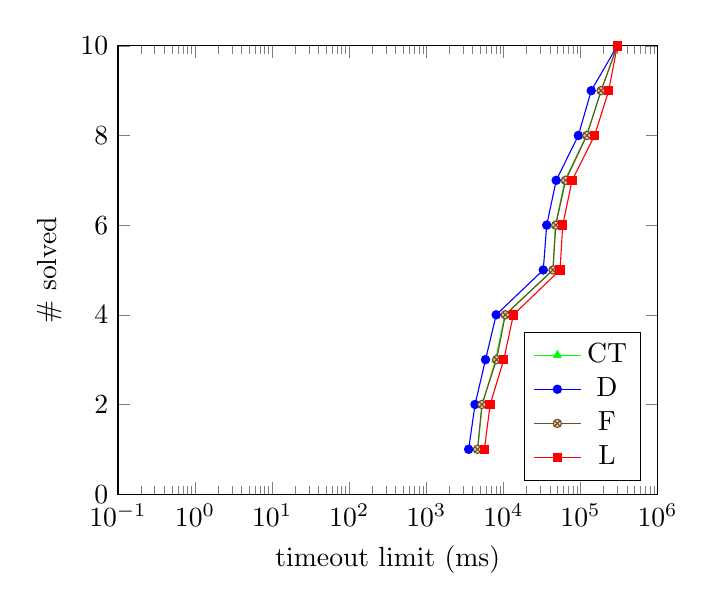
\begin{tikzpicture}[scale=1.0]
  \begin{axis}[
    xmode=log,
    ymin=0,ymax=10,
    xmin=0.1, xmax=1000000,
    every axis plot/.style={thin},
    xlabel={timeout limit (ms)},
    ylabel={\# solved},
    legend pos=south east
    % table/create on use/cumulative distribution/.style={
    %   create col/expr={\pgfmathaccuma + \thisrow{f(x)}}   
    % }
    ]
    \addplot 
    [mark=triangle*,
    mark size=1.5,
    mark options={solid},
    green] 
    coordinates {(4643.908, 1)
(5314.612, 2)
(7919.405, 3)
(10457.700, 4)
(43815.687, 5)
(47278.103, 6)
(62742.592, 7)
(119552.113, 8)
(184956.947, 9)
(300000.177, 10)};

    \addplot 
    [blue,
    mark=*,
    mark size=1.5,
    mark options={solid}]
    coordinates {(3538.073, 1)
(4284.986, 2)
(5862.478, 3)
(8060.677, 4)
(32868.279, 5)
(36463.739, 6)
(48409.543, 7)
(93765.672, 8)
(137802.419, 9)
(300000.168, 10)};

    \addplot [brown!60!black,
    mark options={fill=brown!40},
    mark=otimes*,
    mark size=1.5]
    coordinates {(4612.204, 1)
(5259.809, 2)
(8169.496, 3)
(10583.228, 4)
(43957.885, 5)
(47788.415, 6)
(64135.866, 7)
(120842.255, 8)
(185228.631, 9)
(300000.239, 10)};

    \addplot 
    [red,
    mark size=1.5,
    mark=square*]
    coordinates {(5665.982, 1)
(6731.563, 2)
(10103.827, 3)
(13471.877, 4)
(54252.560, 5)
(58819.370, 6)
(77837.279, 7)
(152362.863, 8)
(232138.799, 9)
(300000.308, 10)};
    \legend{CT,D,F,L}
  \end{axis}
\end{tikzpicture}
